\section*{Porównanie z innymi modelami klasyfikacji obrazów}
W tej sekcji porównamy wyjaśnienia generowane przez XAI dla różnych modeli klasyfikacji obrazów.
Wyjaśnienia te mogą się różnić w zależności od zastosowanego modelu, co wpływa na interpretację wyników i zrozumienie działania modelu.

Jednm z głównych aspektów, który należy uwzględnić przy porównywaniu wyjaśnień z różnych modeli, jest rozdzielczość wyjaśnień generowanych przez GradCAM.
Rozdzielczość ta zależy od wymiarów wyjściowych warstw konwolucyjnych modelu.
W przypdaku modeli o różnych architekturach, takich jak ResNet, VGG czy Inception, wyjściowe wymiary warstw konwolucyjnych mogą się znacznie różnić, co prowadzi do wyjaśnień o różnych pozimach szczegółowości.

W celu oceny spójności wyjaśnień, każda z metod XAI została użyta do wygenerowania wyjjaśnień dla tego samego zestawu obrazów.
Wyniki były przedstwaione za pomocą metryki IoU, która mierzy stopień pokrycia się regionów uznawanych za istotne przez różne metody.

LIME vs SHAP
\begin{figure}
	\centering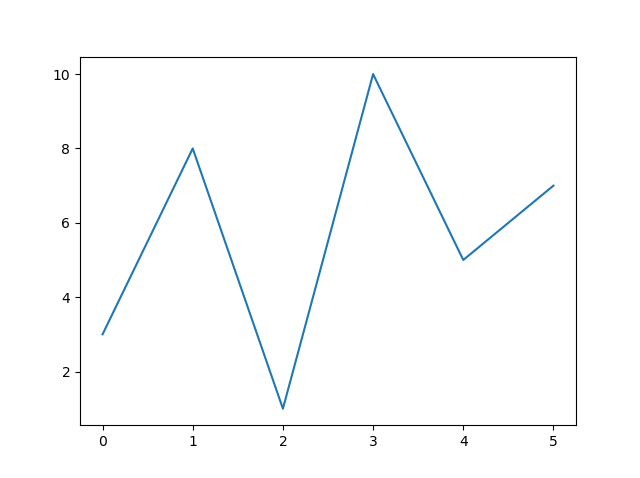
\includegraphics[width=.6\textwidth]{images/example}
	\caption{Sieć dokera \cite{docker_compose_reference}}  \label{rys:network}
\end{figure}

LIME vs GradCAM
\begin{figure}
	\centering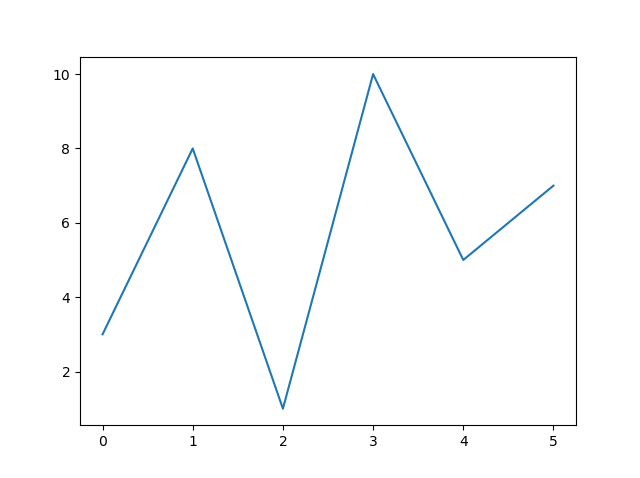
\includegraphics[width=.6\textwidth]{images/example}
	\caption{Sieć dokera \cite{docker_compose_reference}}  \label{rys:network}
\end{figure}

SHAP vs GradCAM
\begin{figure}
	\centering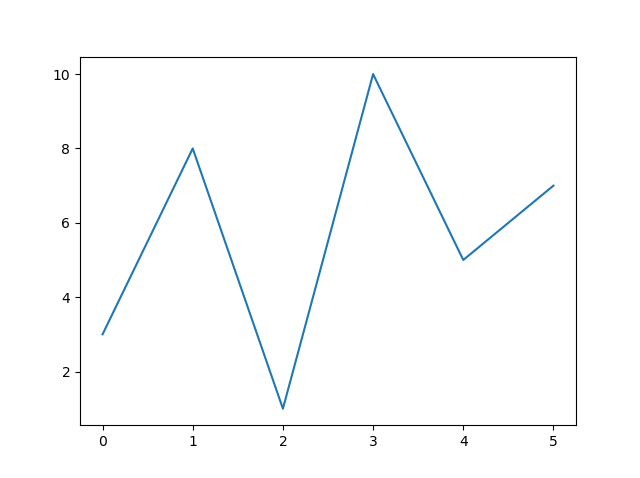
\includegraphics[width=.6\textwidth]{images/example}
	\caption{Sieć dokera \cite{docker_compose_reference}}  \label{rys:network}
\end{figure}

Jak widać spójność jest ...

W tej części przeprowadzimy analizę porównawczą metod XAI na całym zbiorze danych.
Skupimy się na ocenie Intersection over Union oraz zmianach w pewności modelu po zastosowaniu wyjaśnień. Celem jest zrozumienie, jak skutecznie każda metoda identyfikuje istotne cechy obrazu w kontekście całego zbioru.

IoU
\begin{figure}
	\centering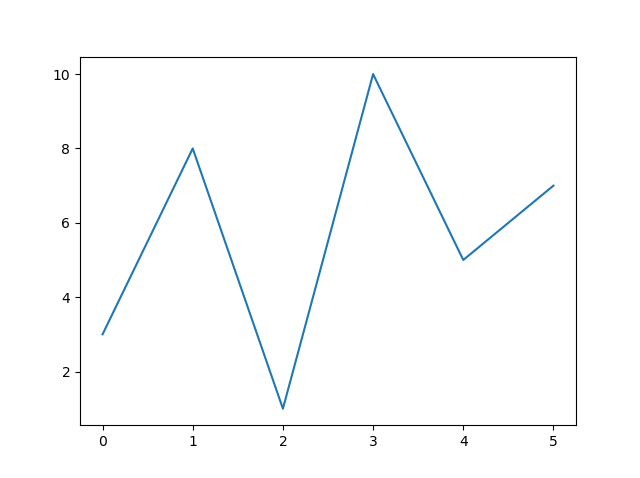
\includegraphics[width=.6\textwidth]{images/example}
	\caption{Sieć dokera \cite{docker_compose_reference}}  \label{rys:network}
\end{figure}

Average Drop in Confidence
\begin{figure}
	\centering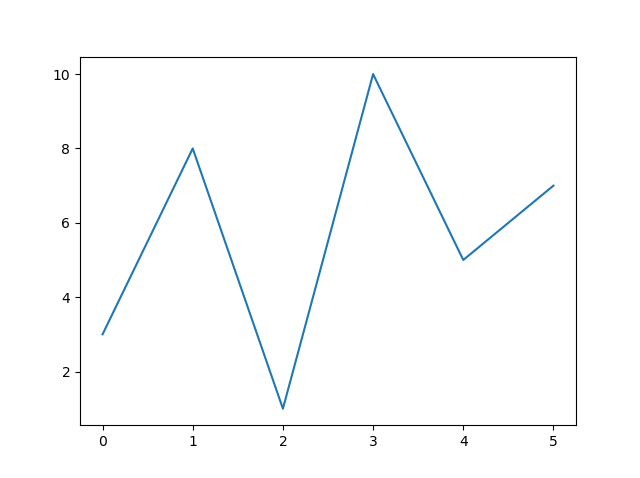
\includegraphics[width=.6\textwidth]{images/example}
	\caption{Sieć dokera \cite{docker_compose_reference}}  \label{rys:network}
\end{figure}

Average Percent Increase in Confidence
\begin{figure}
	\centering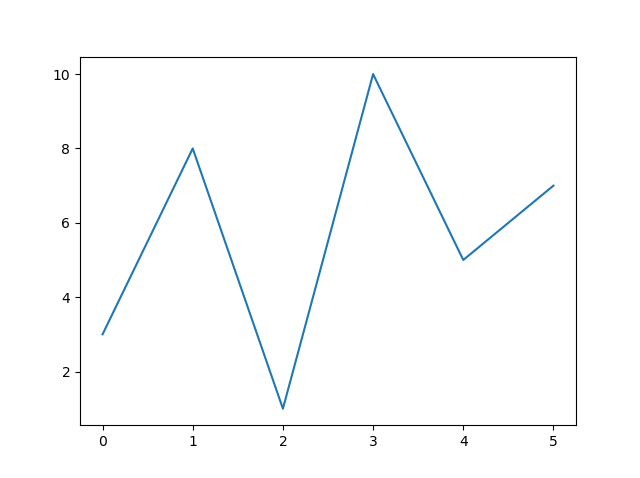
\includegraphics[width=.6\textwidth]{images/example}
	\caption{Sieć dokera \cite{docker_compose_reference}}  \label{rys:network}
\end{figure}

Jak widać ...
